\documentclass{standalone}
\usepackage[dvipsnames]{xcolor}
\usepackage{tikz}
\usetikzlibrary{decorations.pathreplacing,positioning, arrows.meta}

\begin{document}
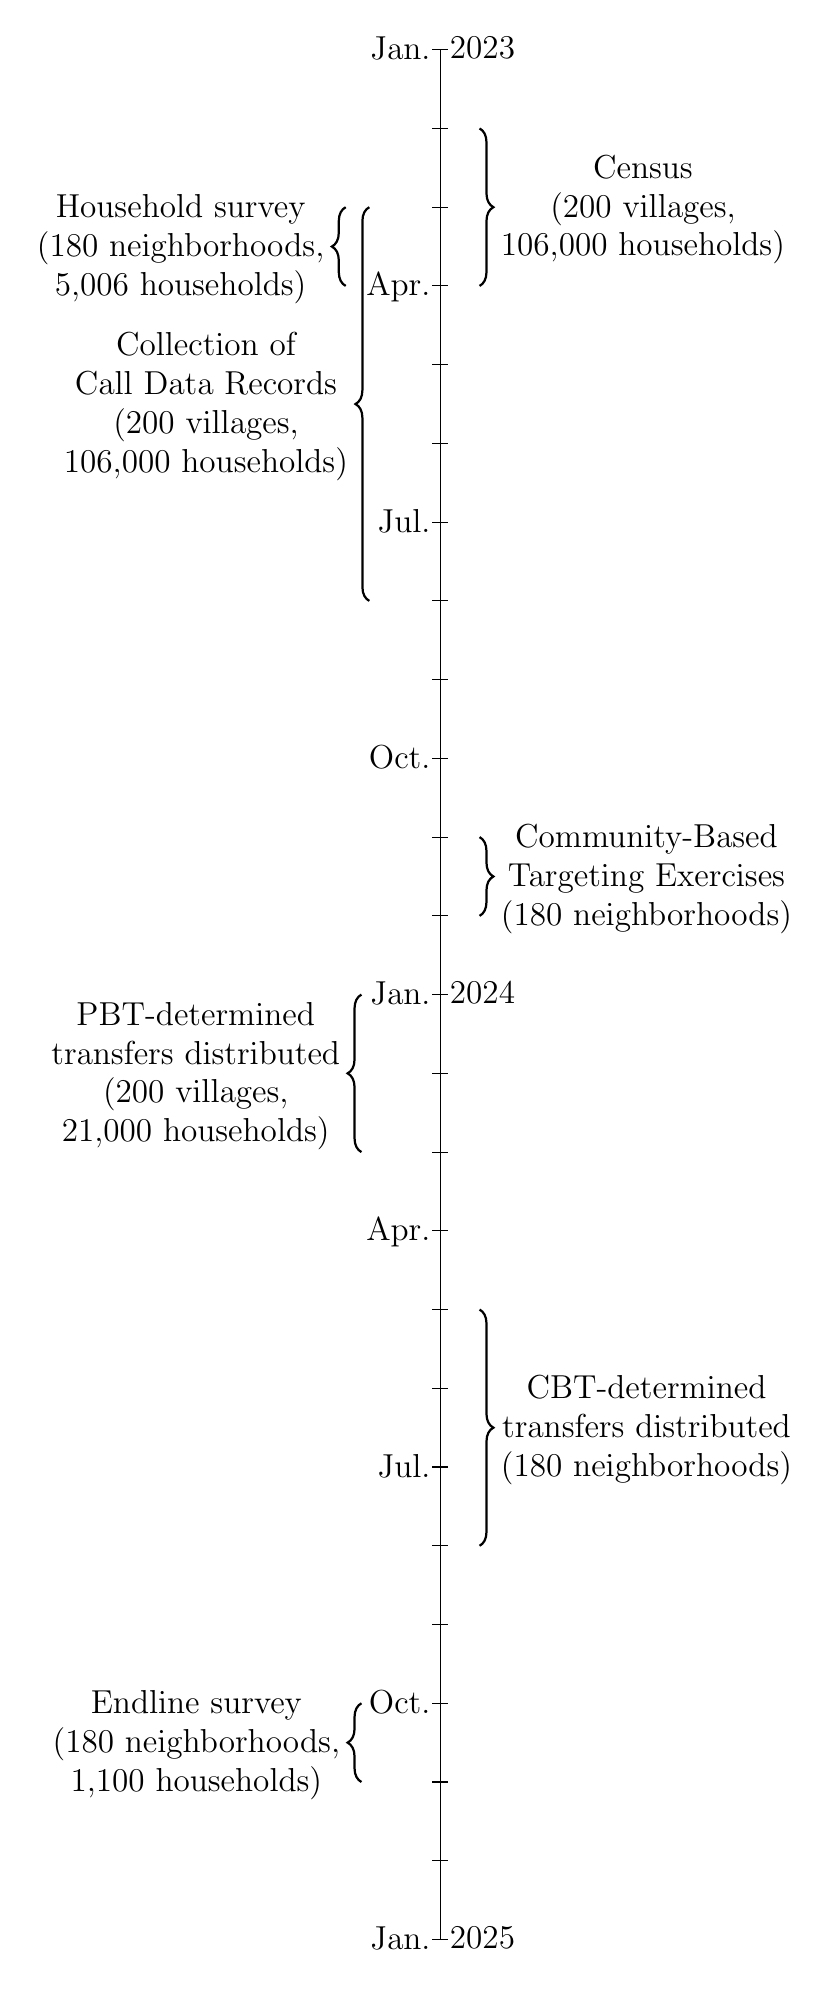
\begin{tikzpicture}[%
    every node/.style={
        font=\large,
        % Better alignment, see https://tex.stackexchange.com/questions/315075
        %text height=1ex,
        text depth=.25ex,
    },
]

% draw vertical line   
\draw[-] (0,0) -- (0,24);

% draw horizontal ticks lines
%\foreach \x in {0,6,...,24}{
%    \draw (3pt, \x cm) -- %(0pt, \x cm);
%}

\foreach \x in {0,1,...,24}{
    \draw (-0.1, \x) -- (0.1, \x);
}

% place axis labels
\node[anchor=east] at (0,24) {Jan.};
\node[anchor=west] at (0,24) {2023};
\node[anchor=east] at (0,21) {Apr.};
\node[anchor=east] at (0,18) {Jul.};
\node[anchor=east] at (0,15) {Oct.};
\node[anchor=east] at (0,12) {Jan.};
\node[anchor=west] at (0,12) {2024};
\node[anchor=east] at (0,9) {Apr.};
\node[anchor=east] at (0,6) {Jul.};
\node[anchor=east] at (0,3) {Oct.};
\node[anchor=east] at (0,0) {Jan.};
\node[anchor=west] at (0,0) {2025};



\draw [thick ,decorate,decoration={brace,amplitude=5pt}] (0.5,23)  -- (0.5,21) 
       node [align=center,black,midway,right=4pt] {Census \\ (200 villages, \\ 106,000 households)};
\draw [thick ,decorate,decoration={brace,mirror,amplitude=5pt}] (-1.2,22)  -- (-1.2,21) 
       node [align=center,black,midway,left=4pt] {Household survey \\ (180 neighborhoods, \\ 5,006 households)};
\draw [thick ,decorate,decoration={brace,mirror,amplitude=5pt}] (-0.9,22)  -- (-0.9,17) 
       node [align=center,black,midway,left=4pt] {Collection of \\ Call Data Records \\ (200 villages, \\ 106,000 households)};
\draw [thick ,decorate,decoration={brace,amplitude=5pt}] (0.5,14)  -- (0.5,13) 
       node [align=center,black,midway,right=4pt] {Community-Based \\ Targeting Exercises \\ (180 neighborhoods)};
       
    
\draw [thick ,decorate,decoration={brace,mirror,amplitude=5pt}] (-1,12)  -- (-1,10) 
       node [align=center,black,midway,left=4pt] {PBT-determined \\ transfers distributed \\ (200 villages, \\ 21,000 households) };       
\draw [thick ,decorate,decoration={brace,amplitude=5pt}] (0.5,8)  -- (0.5,5) 
       node [align=center,black,midway,right=4pt] {CBT-determined \\ transfers distributed \\ (180 neighborhoods)};  
      %anchor=west, 
\draw [thick ,decorate,decoration={brace,mirror,amplitude=5pt}] (-1,3)  -- (-1,2) 
       node [align=center,black,midway,left=4pt] {Endline survey \\ (180 neighborhoods, \\ 1,100 households)};  

\end{tikzpicture}
\end{document}

